\documentclass[12pt, openany]{report}

\LoadClass[12pt,french]{book}
\RequirePackage[paperheight=29.7cm, paperwidth=21cm,
%includehead,
nomarginpar,
textwidth=18cm,
textheight=23cm,
headheight=1.5cm,
lmargin=2cm,
rmargin=2cm,
%showframe,
]{geometry}

\RequirePackage{lastpage}

%\renewcommand{\section}{%
%	\@startsection
%	{section}{1}{0pt}{-1.5ex plus -1ex minus -.2ex}%
%	{1ex plus .2ex}{\large\sffamily\slshape\headlinecolor}%
%}
%

\newcommand{\headlinecolor}{\normalcolor}
\RequirePackage{xcolor}

\RequirePackage{tikz}

\RequirePackage[utf8]{inputenc}
\RequirePackage[T1]{fontenc}
\RequirePackage{framed,eso-pic,graphicx,url}

%2024 inutile \RequirePackage[french]{babel}


%headers et footers avec FancyHeader
\RequirePackage{fancyhdr}
\pagestyle{fancy}

\lhead{{\small \auteurA \ \auteurB \ \auteurC}}
\rhead{Projet <<\ Algorithmique et complexité\ >>}
\chead{}
\lfoot{{\small \textit{\sujet}}}
\rfoot{\textsf{\small{\thepage}}}%/\pageref{LastPage}}}}
\cfoot{}

%%"boîte" colorée pour le sujet de la page de garde
\RequirePackage{tcolorbox}

%pour les matrices et les notations mathématiques
\RequirePackage{amsmath}

%%URL et lien dasn le texte
\RequirePackage{hyperref}
\RequirePackage{url}

%%au besoin
\RequirePackage{verbatim}

%%pour les figures et subfigures
\RequirePackage{caption}
\RequirePackage{subcaption}

%%listings
\RequirePackage{listings}
\lstset{language=caml, breaklines=true,
	backgroundcolor=\color{pastelgray},
	fillcolor=\color{white},
	rulesepcolor=\color{black},
	rulecolor=\color{gray},
	columns=fullflexible,
	showstringspaces=false,          % underline spaces within strings only
	%framesep=14pt,
	%framerule=0pt,
	showspaces=false,                % show spaces everywhere adding particul
	numbers=left,                   % where to put the line-numbers; possible values are (none, left, right)
	%numbersep=5pt,                   % how far the line-numbers are from the code
	numberstyle=\tiny\color{black}, % the style that is used for the line-numbersframe=single,
	basicstyle=\footnotesize\ttfamily,
	frame=shadowbox,
	frameround=tttt,
	keywordstyle=\bfseries\color{olive},
	commentstyle=\itshape\color{purple},
	identifierstyle=\color{blue},
	stringstyle=\color{orange},
	literate=
	{á}{{\'a}}1 {é}{{\'e}}1 {í}{{\'i}}1 {ó}{{\'o}}1 {ú}{{\'u}}1
	{Á}{{\'A}}1 {É}{{\'E}}1 {Í}{{\'I}}1 {Ó}{{\'O}}1 {Ú}{{\'U}}1
	{à}{{\`a}}1 {è}{{\`e}}1 {ì}{{\`i}}1 {ò}{{\`o}}1 {ù}{{\`u}}1
	{À}{{\`A}}1 {È}{{\'E}}1 {Ì}{{\`I}}1 {Ò}{{\`O}}1 {Ù}{{\`U}}1
	{ä}{{\"a}}1 {ë}{{\"e}}1 {ï}{{\"i}}1 {ö}{{\"o}}1 {ü}{{\"u}}1
	{Ä}{{\"A}}1 {Ë}{{\"E}}1 {Ï}{{\"I}}1 {Ö}{{\"O}}1 {Ü}{{\"U}}1
	{â}{{\^a}}1 {ê}{{\^e}}1 {î}{{\^i}}1 {ô}{{\^o}}1 {û}{{\^u}}1
	{Â}{{\^A}}1 {Ê}{{\^E}}1 {Î}{{\^I}}1 {Ô}{{\^O}}1 {Û}{{\^U}}1
	{Ã}{{\~A}}1 {ã}{{\~a}}1 {Õ}{{\~O}}1 {õ}{{\~o}}1
	{œ}{{\oe}}1 {Œ}{{\OE}}1 {æ}{{\ae}}1 {Æ}{{\AE}}1 {ß}{{\ss}}1
	{ű}{{\H{u}}}1 {Ű}{{\H{U}}}1 {ő}{{\H{o}}}1 {Ő}{{\H{O}}}1
	{ç}{{\c c}}1 {Ç}{{\c C}}1 {ø}{{\o}}1 {å}{{\r a}}1 {Å}{{\r A}}1
	{€}{{\euro}}1 {£}{{\pounds}}1 {«}{{\guillemotleft}}1
	{»}{{\guillemotright}}1 {ñ}{{\~n}}1 {Ñ}{{\~N}}1 {¿}{{?`}}1
}



\setcounter{secnumdepth}{2}
\setcounter{chapter}{1}

% % % % % % % % % % % % % % % %
% http://latexcolor.com/
% % % % % % % % % % % % % % % %
\definecolor{bleudefrance}{rgb}{0.19, 0.55, 0.91} %Bleu de France #318CE7
\definecolor{pastelgray}{rgb}{0.93, 0.93, 0.93}
% % % % % % % % % % % % % % % %
% http://ethanschoonover.com/solarized
% % % % % % % % % % % % % % % %
\usepackage[utf8]{inputenc}
\usepackage[T1]{fontenc}
\usepackage[a4paper,left=2cm,right=2cm,top=2cm,bottom=2cm]{geometry}
\usepackage[frenchb]{babel}
\usepackage{libertine}
\usepackage[pdftex]{graphicx}
\usepackage{lingmacros}
\usepackage{mdframed}

%Définitions des auteurs
\newcommand{\auteurA}{Elio GENCE}
\newcommand{\auteurB}{Guillaume BELDILMI}

%Définition du sujet
\newcommand{\sujet}{Sujet n°4 : Eternity II}

%% Définitions pour le projet
\title{\LARGE{\titreGeneral}}%ne pas modifier
\author{\auteurA \\ \auteurB}% à modifier selon le nombre d'auteurs

\date{2023-24}

\begin{document}
\setlength{\parindent}{1cm}%ne pas modifier
%\setlength{\parskip}{1ex plus 0.5ex minus 0.2ex}

%%Page de garde rapport Master Info Algo et Complexité
%%RRaffin, 01/01/2023

\begin{titlepage}
%%Bordure
\AddToShipoutPicture*{%
	\setlength\unitlength{1mm}
	\put(0,0){\makebox(0,0)[lb]{\color{white}\rule{\paperwidth}{\paperheight}}}
	\put(0,0){\makebox(0,0)[lb]{\color{bleudefrance}\rule{25mm}{\paperheight}}}
	\put(15,190){\rotatebox{90}{%
		\makebox(0,0)[r]{\fontsize{30}{30}\color{orange!50!white}
		\bfseries \selectfont{Algorithmique et complexité M1}}}
	}
}

%%Logos

\includegraphics[height=2cm]{img/logo-ub.png}
\hfill

\includegraphics[height=2cm]{img/logo-ufr.png}

%%Université/UFR/IEM
\vspace{1cm} 
{\large{Université de Bourgogne, UFR Sciences et Techniques, Département I.E.M.}\par}

%%Titre
\vspace{2cm}
{\huge\bfseries Projet <<\ Algorithmique et complexité\ >>}\par

\vspace{2cm}
\mdfdefinestyle{mdframedStyle}{leftmargin=2cm,rightmargin=2cm,%
	innerleftmargin=0.5cm,innerrightmargin=1cm,%
	frametitlerule=true, frametitlebackgroundcolor=lightgray!50,userdefinedwidth=.8\textwidth,align=center}
\begin{mdframed}[style=mdframedStyle, frametitle={Groupe}]
\begin{large}
	\begin{itemize}
		\item [] \auteurA
		\item [] \auteurB
	\end{itemize}
\end{large}
\end{mdframed}

\vspace{2cm}

%%Sujet

\begin{center}
\begin{tcolorbox}[text width=0.8\textwidth]
\large \sujet
\end{tcolorbox}
\end{center}


\vfill
{\hfill\large 2023-2024\par}

\end{titlepage}


%ne pas modifier

\tableofcontents
\newpage

\section*{Présentation du projet}

Eternity II est un jeu de puzzle inventé par Christopher Monckton en
2007. Le but du jeu est de placer des pièces de puzzle de manière à
ce que les couleurs des bords des pièces soient identiques aux
couleurs des bords adjacents.  Les pièces sont carrées et chaque
côté est coloré. Les pièces sont placées sur une grille de taille
$n \times n$.

Notre projet était de créer un solveur capable de résoudre des
puzzles d’Eternity II de taille 12 par 12 avec une dizaine de
couleurs. Nos seules contraintes étaient que notre programme devait
être écrit en Ocaml et que la résolution devait se faire par une
méthode de recherche arborescente avec retour en arrière (backtrack).

Pour cela, nous avons divisé le projet en plusieurs étapes :
tout d’abord, nous avons créé une structure de données pour
représenter les pièces et la grille. Ensuite, nous avons créé un
ensemble de fonctions permettant de générer un puzzle aléatoire,
de mélanger les pièces du puzzle, et enfin de résoudre le puzzle.
A cela s’ajoute une autre fonction permettant d'afficher le puzzle
afin d'avoir un retour sur l'exécution du programme.

\section*{Organisation}

Premièrement, nous avons réalisé un prototype conformément à
l'ISO-1664 dans un langage plus abordable, Python. Ce prototype
nous a permis de mieux comprendre le problème et de définir
l'architecture de notre programme.

Ensuite, nous avons transcrit ce prototype en Ocaml, en corrigeant
quelques erreurs et en ajoutant des fonctionnalités précédemment
omises après avoir pris en compte le retour du corps enseignant.

Nous avons ensuite testé notre programme sur des puzzles
progressivement de plus en plus grands.

Enfin, nous avons peaufiné notre programme en simplifiant le code
et en corrigeant l'affichage du puzzle afin de rendre le résultat
plus facile à manipuler.

\section*{Explication de l'algorithme utilisé}

Nous avons utilisé un algorithme naïf de backtracking pour résoudre
le puzzle. L’idée est de placer chaque pièce sur la grille en
progressant selon le sens d’écriture. Si une pièce ne peut pas être
placée, on revient à la pièce précédemment placée et on essaie une
autre pièce. Si aucune pièce ne peut être placée, on revient à la
pièce précédente, et ainsi de suite jusqu’à ce que le puzzle soit
résolu. Une fois le puzzle résolu, on affiche le résultat et puis
le programme poursuit son exécution afin de trouver d'autres
solutions. 

D'autres algorithmes plus performants existent, optimisants notamment
l'ordre de placement des pièces (commençant par les pièces de bords
puis progressant vers le centre en zigzag ou en spirale), mais nous
avons choisi de rester sur un algorithme simple pour des raisons de
simplicité et de temps.

Nous avons pour notre faire 2 versions différentes : une avec rotation de pièce et une autre sans.

\subsection*{Analyse de la complexité}


\section*{Explication détaillés (code sans Rotation)}

Pour notre code, nous pouvons le diviser en 5 parties : 
- définition d'une pièce \ref{code:tile}
- creation des structures et initialisation \ref{code:init_board} 
- test de pièce lors du backtrack \ref{code:test_tile} 
- backtrack \ref{code:test_tile} 
- affichage du résultat \ref{code:test_tile} 

\lstinputlisting[inputpath=sources/, caption=Déclaration pièce  (\lstname), label=code:tile]{tile.ml} 

Nous utilisons dans notre code 2 structures : board et tiles.
Board est un tableau de tableau de pièce, il représente le plateau de jeu sur lequel on va venir placer les pièces pour essayer de résoudre le puzzle. 
Tiles quant à lui est un tableau de pièce, il va servir à stocker la liste de pièce encore non placé sur le board.
(à noter que si une pièce identifiant est égal à -1 alors on considère l'emplacement comme vide)

L'initialisation du board ce fait avec un parcours de haut en bas et de gauche à droite/droite à gauche une ligne sur deux (afin de simuler un parcours en zigzag dans les algorithmes de backtrack optimal)
Lors de la création d'un pièce nous avons donc besoin de vérifier seulement 3 paramètres : 
- s'il est adjacent à une bordure (si c'est le cas le/les cotés adjacent prennent la valeur 0)
- la valeur du coté inférieur de la pièce supérieur
- la valeur du coté gauche de la pièce à droite (ou inverse pour un parcours de droite à gauche)
- le reste des coté prendront une valeur aléatoire parmis celle disponible (défini au tout début du code pour une modification rapide)
\lstinputlisting[inputpath=sources/, caption=Initialisation du board (\lstname), label=code:init_board]{init_board.ml} 

Pour ce qui est du test des tuiles lors du backtrack voici le code et ce qui est testé
\lstinputlisting[inputpath=sources/, caption=Test de compatibilité des pièces (fonction imbriqués)(\lstname), label=code:test_tile]{test_tile.ml} 

Le backtrack la partie la plus important est également la partie la plus simple, le test s'occupant du principal tout ce qui reste à faire maintenant est de gérer les boucles de recherches et les appels récurssifs. 
\lstinputlisting[inputpath=sources/, caption=Backtrack (fonction principale) (\lstname), label=code:backtrack]{backtrack.ml} 

Enfin il ne nous reste plus que l'affichage qui est composé de plusieurs boucles imbriqués afin d'obtenir un affichage facilement lisible 
\lstinputlisting[inputpath=sources/, caption=Affichage du résultat (board)(\lstname), label=code:print]{print.ml} 

\subsection*{Explication détaillés (code avec Rotation)}

L'algorithme avec rotation est très similaire cependant dans le backtrack \ref{code:backtrack} et dans le test de pièce \ref{code:test_tile} on rajoute un nouveau paramètre (que l'on nomme k) variant entre 0 et 3 afin de pouvoir tester chaque rotation et ainsi obtenir de nouvelle solution.

\lstinputlisting[inputpath=sources/, caption=Paramètre k pour savoir le sens de rotation de la pièce (\lstname), label=code:rotation]{rotation.ml}

Ainsi toutes les solutions possibles seront obtenus mais cela entraine 2 problème :
La durée -> le code est bien plus long car bien plus de solution à tester
Les solutions -> Le nombre de solution obtenus peux en réalité être divisé par 4 car nous trouvons des solutions "doublons" que l'on peut retrouver simplement en tournant le plateau de puzzle. Une solution possible à se problème serait de fixer un coin et de faire le backtrack à partir de ce moment la.

\section*{Résultats et analyses}

\subsection*{Temps}

Voici les temps observé pour un code sans rotation :
\begin{figure}
  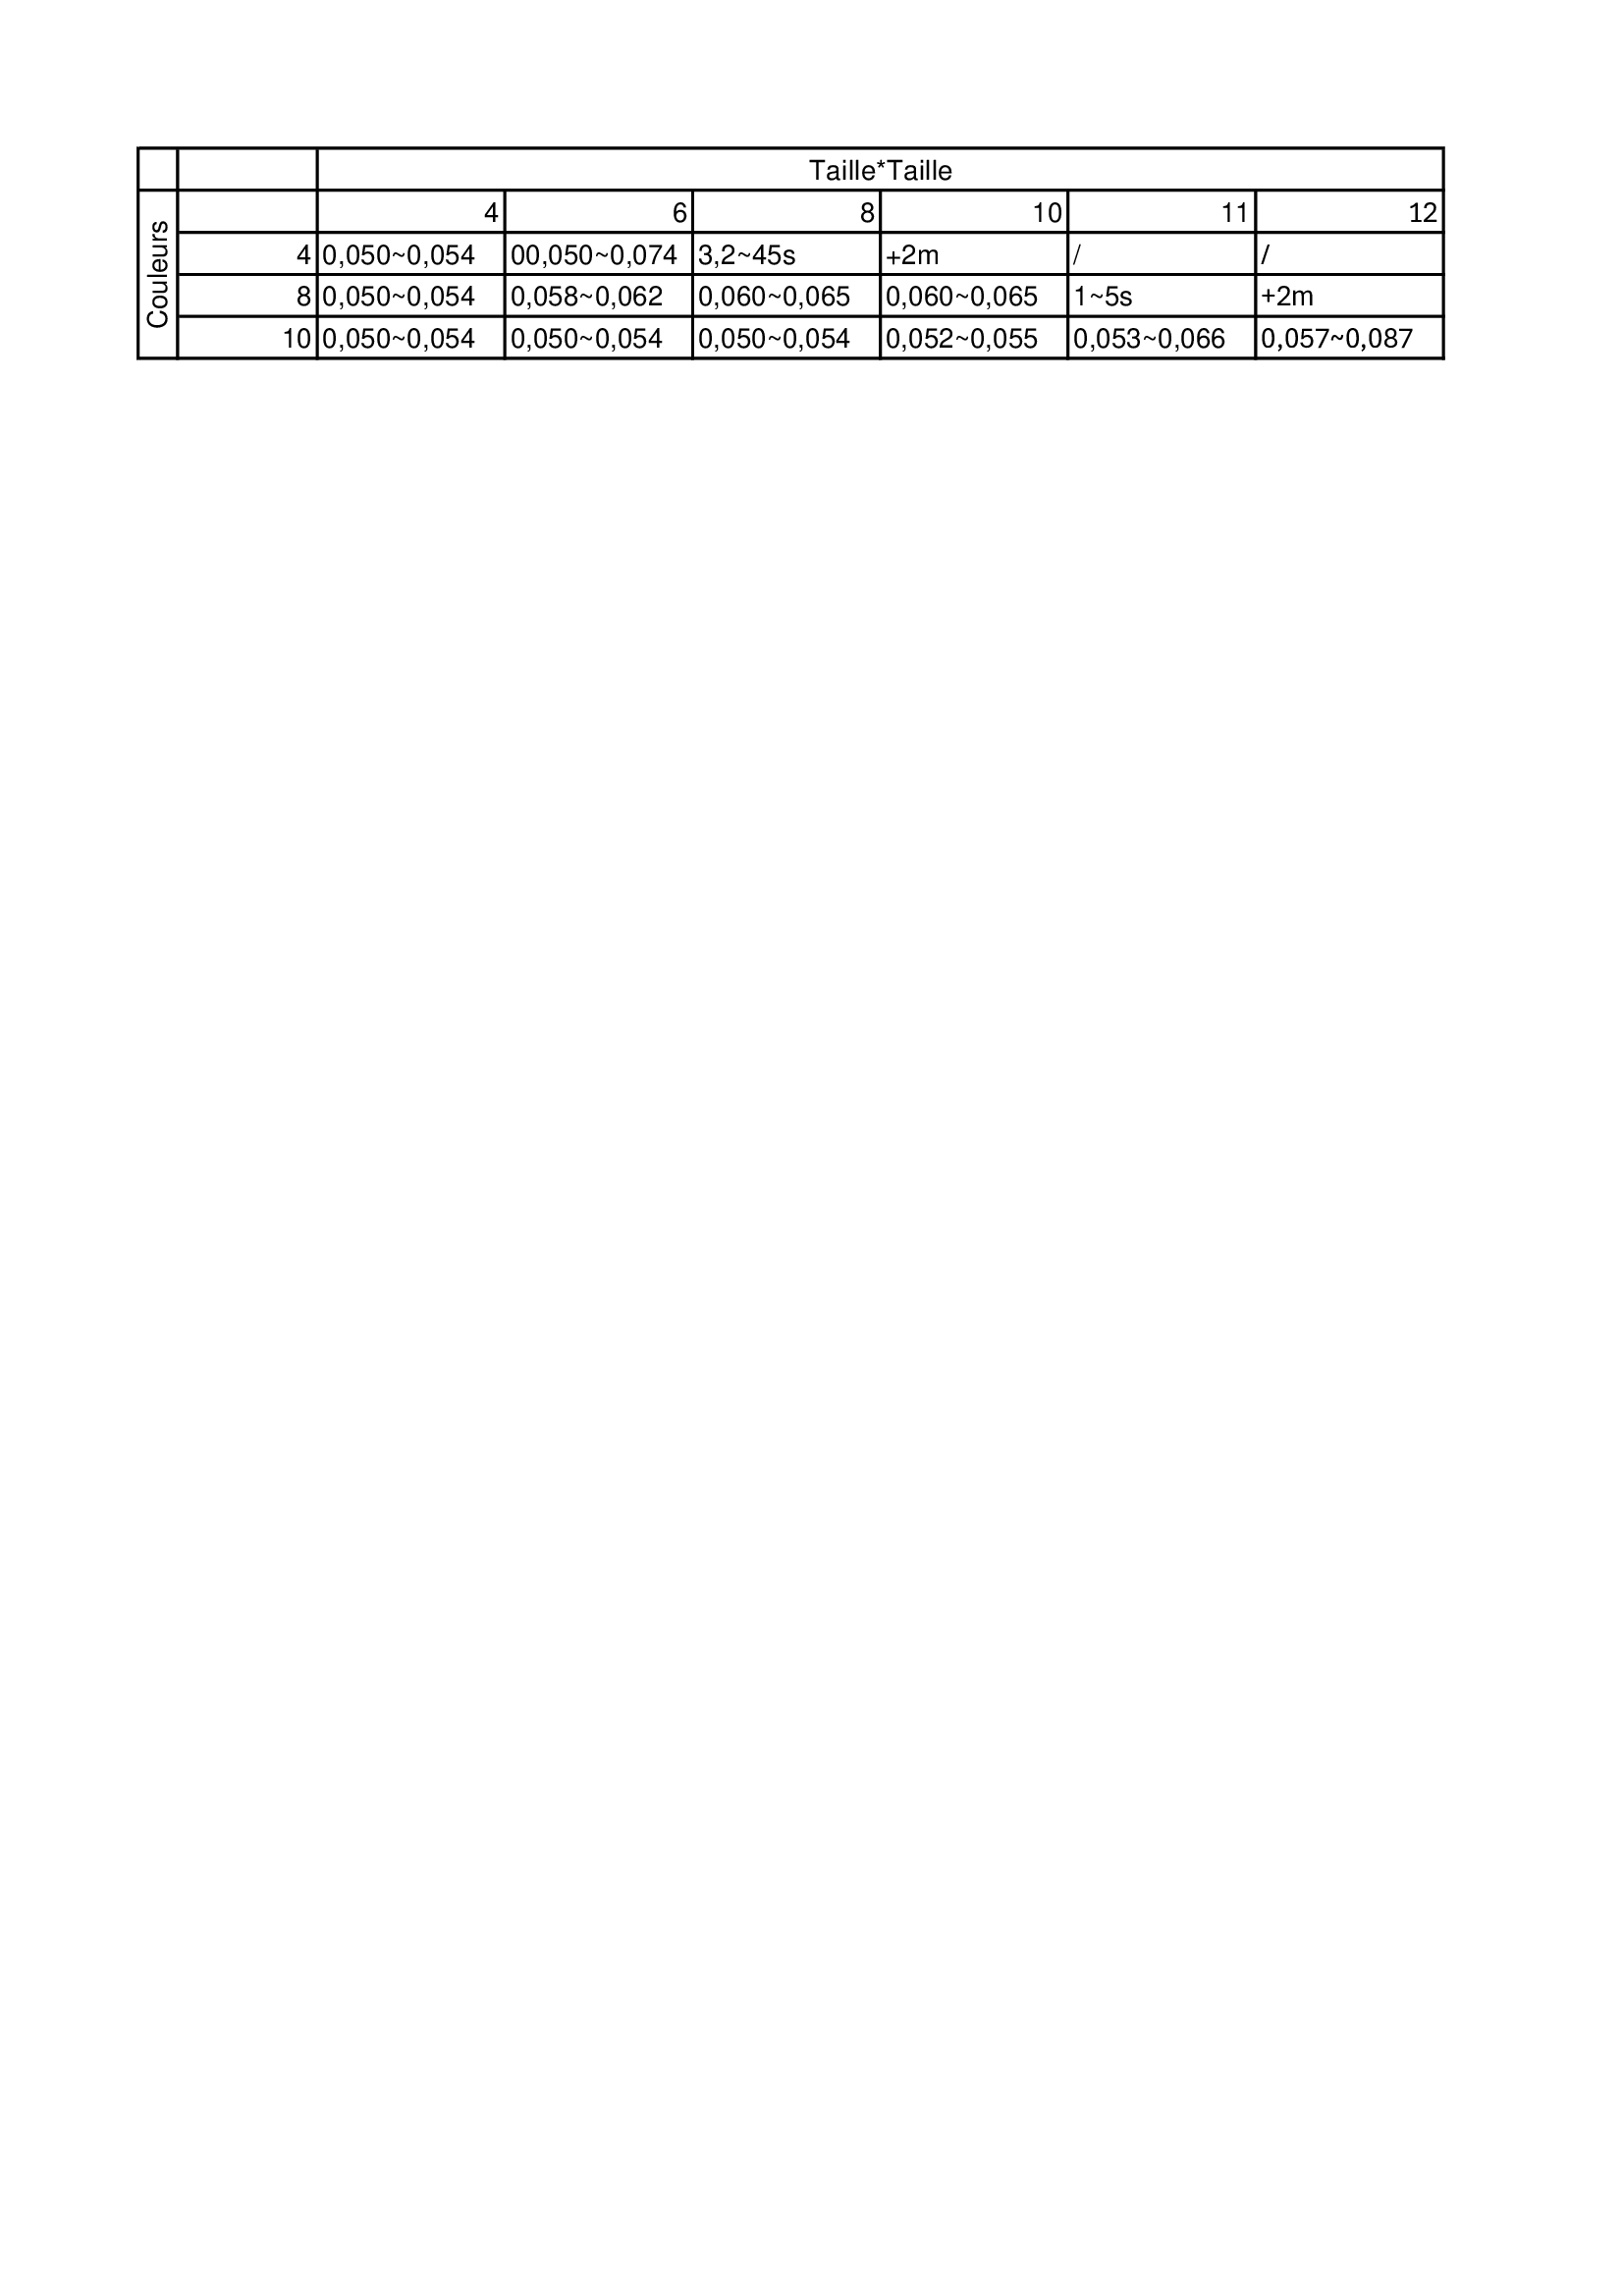
\includegraphics[width=\linewidth]{img/TimeNR.png}
  \caption{Temps sans rotation}
  \label{img:timeNR}
\end{figure}
Comme on peux le constater la durée moyenne varie selon le nombre de couleur et la taille (logique). Cependant le temps varie de facon différente. Tandis que le temps se rallonge lorsque l'on augmente la taille, il diminue au contraire quand le nombre de couleur augmente. C'est logique car le nombre de cas à tester et de solution possible diminue lorsque le nombre de couleurs augmentent, si toute les pièces sont très atypiques alors il deviens plus dur de les subsituer à l'inverse si les pièces se ressemblent (aka le nombre de couleur est faible) alors le programme va devoir tester bien plus de possibilité de résolution car les pièces vont s'imbriquer plus facilement les unes dans les autres.

Voici les temps observé pour un code avec rotation :
\begin{figure}
  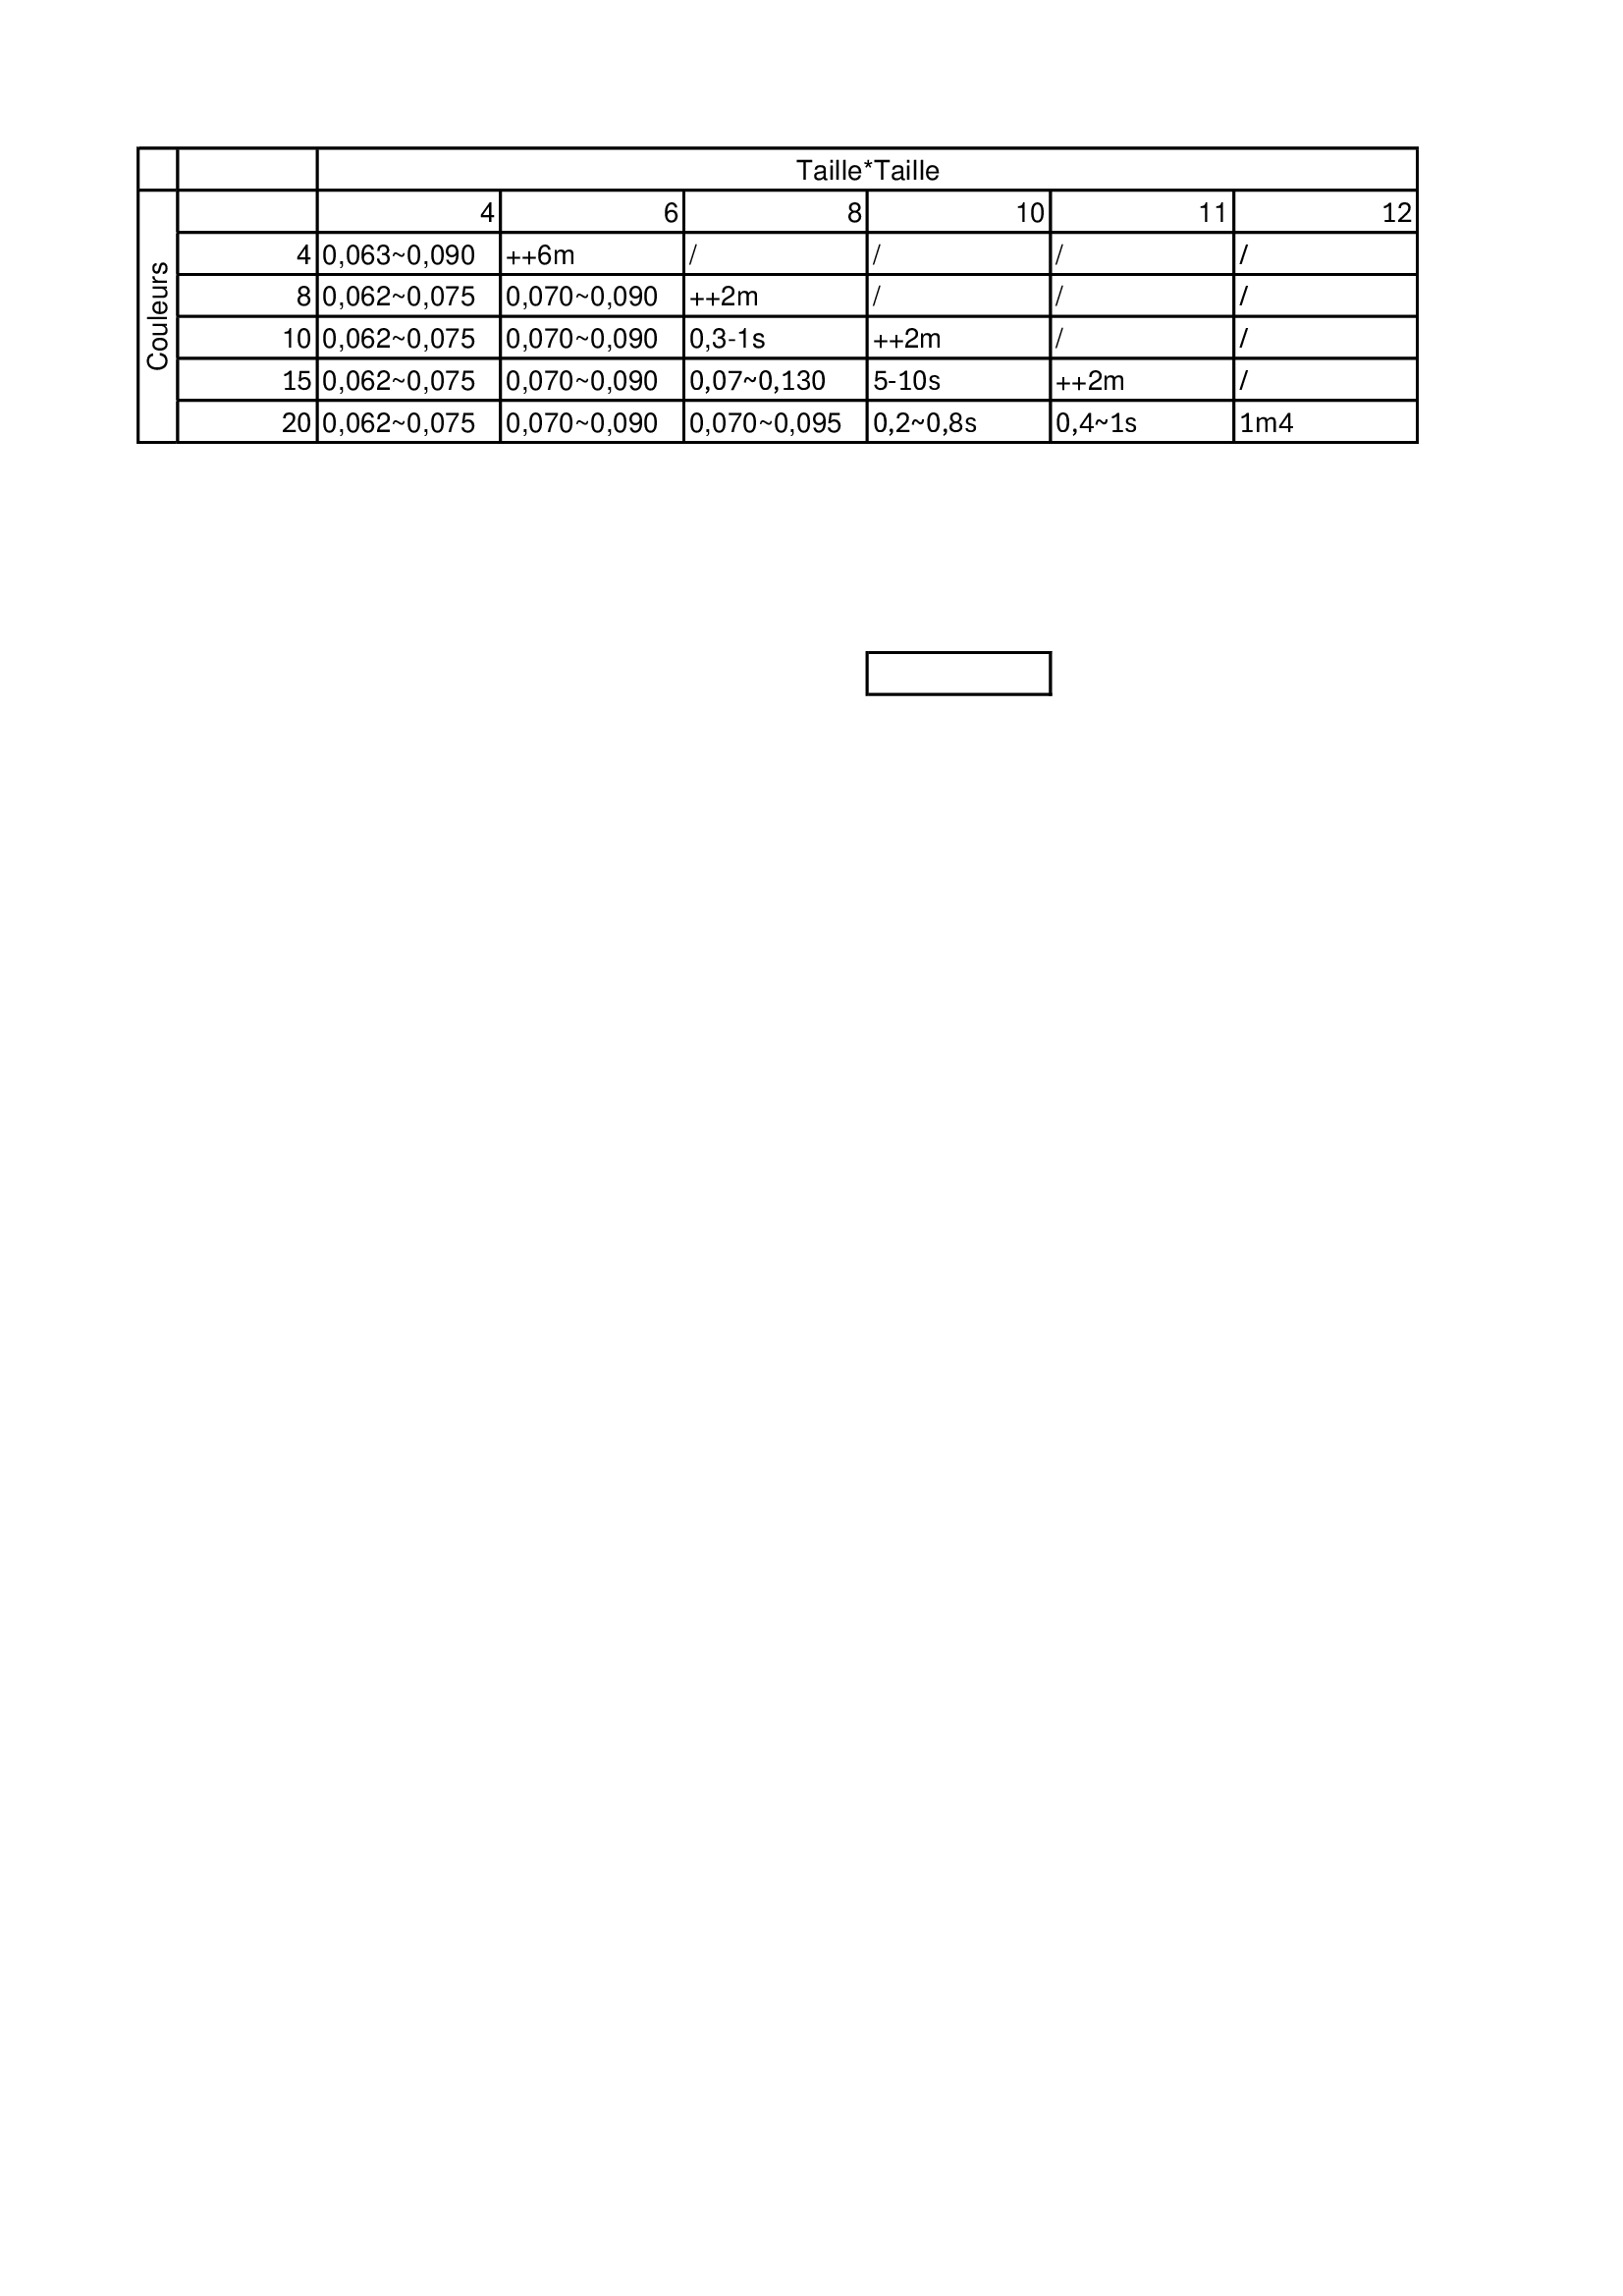
\includegraphics[width=\linewidth]{img/TimeR.png}
  \caption{Temps avec rotation}
  \label{img:timeR}
\end{figure}
Nous observons ici le même phénomène qu'avec le code sans rotation cependant les temps sont bien plus car, contrairement au précédent code, chaque pièce doit être tester 4 fois (une dans chaque sens) rendant la recherche plus fastidieuse mais également en augmentant le nombre de solution possible ! 

\subsection*{Affichage}

Voici un exemple de puzzle de taille 5 par 5 avec 5 couleurs résolu
par notre programme sans rotation :
\begin{verbnobox}\fontsize{7pt}{7pt}\selectfont
  \VerbatimInput{sources/resNR_5x5.txt}
\end{verbnobox}

Voici un exemple de puzzle de taille 5 par 5 avec 5 couleurs résolu
par notre programme avec rotation :
\begin{verbnobox}\fontsize{7pt}{7pt}\selectfont
  \VerbatimInput{sources/resR_5x5.txt}
\end{verbnobox}
Comme dis lors de l'explication, nous obtenons tous les résultats dans 4 rotations possibles donc il faut diviser par 4 le nombre de résultat obtenus pour avoir le nombre réel de solutions possibles (un code prennant en compte ce détail sera ajouter en annexe \ref{codeComplet:RotationTileLocked}


\section*{Conclusion}
% une conclusion qui établit (ou non) en justifiant le lien entre votre implé-
% mentation et l’analyse théorique de l’algorithme

\section*{Annexe}

\lstinputlisting[inputpath=sources/, caption=Paramètre k pour savoir le sens de rotation de la pièce (\lstname), label=code:rotation]{rotation.ml}

COPIER TOUT LES CODES, PYTHON AUSSI ???

\end{document}
